\section*{Question 1}
\fakesection{1}

Consider the Z-transform of the impulse response of a causal FIR filter of order $M$:
\begin{align}
    H(z) = \sum_{n=0}^{M} h[n] z^{-n}
\end{align}
If the filter is linear phase, then the coefficients $h[n]$ must either be symmetric or antisymmetric.

We first consider the case of symmetric coefficients, for which $h[n]=h[M-n]$. If we substitute $n=M-n$, or equivalently $-n=n-M$, into the exponent of $z$ in (1.1), we obtain
\begin{align}
    H(z) = \sum_{n=0}^{M} h[n] z^{n-M}
         = z^{-M} \sum_{n=0}^{M} h[n] z^n
         = z^{-M} \left(H(z^{-1})\right)
\end{align}
Now considering the case of antisymmetric coefficients, for which $h[n]=-h[M-n]$, we find
\begin{align}
    H(z) = \sum_{n=0}^{M} -h[n] z^{n-M}
         = -z^{-M} \sum_{n=0}^{M} h[n] z^n
         = -z^{-M} \left(H(z^{-1})\right)
\end{align}
The results (1.2) and (1.3) can be combined as the following single expression:
\begin{align}
    H(z) = \pm z^{-M} \left( H(z^{-1}) \right)
\end{align}
By definition, the zeros of the filter response are the values of $z$ satisfying $H(z)=0$. Per (1.4), this also implies $\pm z^{-M} H(z^{-1})=0$. Assuming $|z|\neq 0$, it must be true that $H(z^{-1})=0$. The significance of this result is that if $z$ is a zero, then its reciprocal $z^{-1}$ is also a zero.

Furthermore, if the filter coefficients $h[n]$ are real-valued, then the following is true of $H(z^*)$, where $z^*$ is the complex conjugate of $z$:
\begin{align}
    H(z^*) = \sum_{n=0}^{M} h[n] (z^*)^{-n}
           = \sum_{n=0}^{M} h[n] (z^{-n})^*
           = \left(H(z)\right)^*
\end{align}
The property $(z^*)^k=(z^k)^*$ for arbitrary $k$ can easily be proven by expressing $z$ as $e^{j\theta}$:
\begin{align}
    (z^*)^k = (e^{-j\theta})^k = e^{-jk\theta} = (e^{jk\theta})^* = (z^k)^*
\end{align}
and since $h[n]$ are real, multiplying $h[n]$ by either $(z^*)^{-n}$ or $(z^{-n})^*$ scales the magnitude equally in both cases and does not change the phase. Therefore, result (1.5) signifies that if $z$ is a zero (i.e. $H(z)=0$), then its conjugate $z^*$ is also a zero.

\newpage

We are now in a position to exhaustively enumerate all possible patterns of zeros by considering all possible cases of $z$.
\begin{enumerate}[label=(\roman*)]
    \item Consider $z=1$. A zero at $z=1$ is its own reciprocal and has no complex conjugate, so the first pattern is a single zero at $z=1$.

    \item Consider $z=-1$. A zero at $z=-1$ is also its own reciprocal and has no complex conjugate, so the second pattern is a single zero at $z=-1$.

    \item Consider $z\in\mathbb{R},z\neq\pm 1$. Any real-valued zero except $\pm 1$ has a real-valued reciprocal and no complex conjugate, so the third pattern is a real reciprocal pair: $z$ and $z^{-1}$.

    \item Consider $z\in\mathbb{C},|z|=1$. The reciprocal of a complex number of magnitude unity is equal to its conjugate; so, representing $z$ as $e^{j\theta}$, the fourth pattern is a complex reciprocal pair on the unit circle: $z=e^{j\theta}$ and $z^{-1}=e^{-j\theta}$.

    \item Consider $z\in\mathbb{C},|z|\neq 1$. For a complex number of non-unity magnitude, its conjugate, reciprocal, and reciprocal conjugate are distinct; so, representing $z$ as $re^{j\theta}$, the final pattern is a complex reciprocal conjugate quad: $re^{j\theta}$, $re^{-j\theta}$, $\frac{1}{r}e^{j\theta}$, and $\frac{1}{r}e^{-j\theta}$.
\end{enumerate}

\bigskip

Figure \ref{fig:zero_patterns} visualises examples of each zero pattern on and around the unit circle.

\begin{figure}[ht]
    \centering
    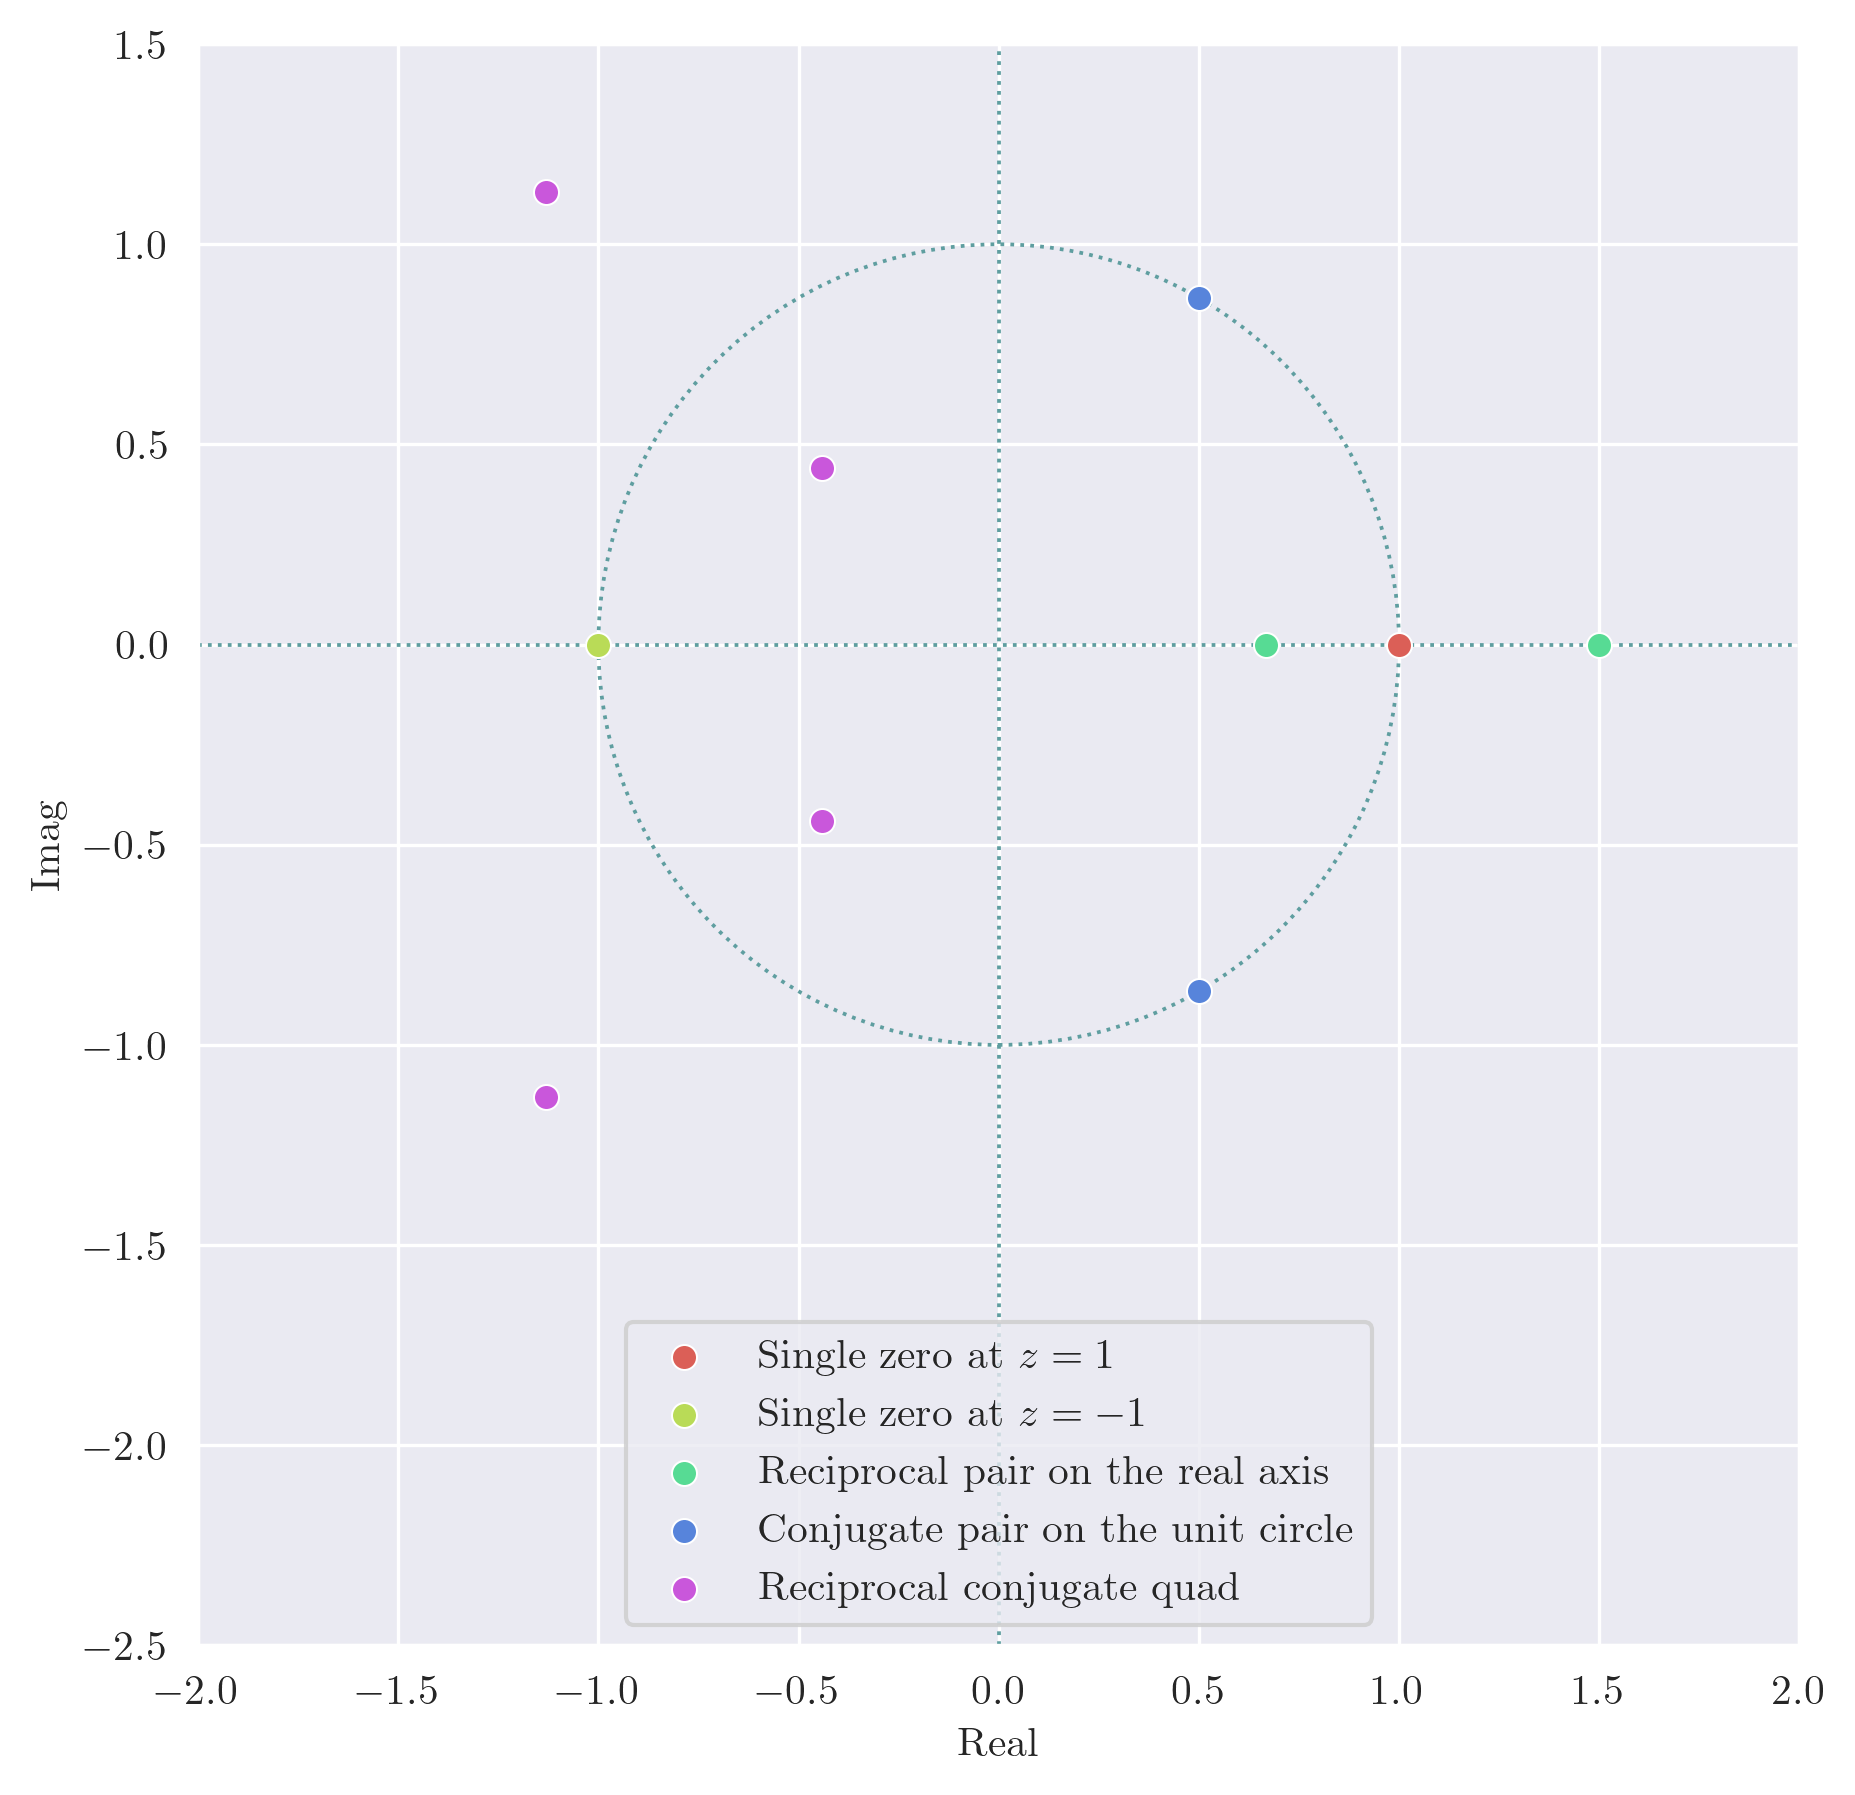
\includegraphics[width=0.9\textwidth]{images/q1_zero_patterns.png}
    \caption{Possible zero patterns for real-valued, linear phase FIR filter}
    \label{fig:zero_patterns}
\end{figure}
